\documentclass[a4paper,11pt]{article}

\usepackage{a4wide}
\usepackage{microtype}
\usepackage[utf8]{inputenc}
\usepackage[ngerman]{babel}
\usepackage[default,light,semibold]{sourceserifpro}
\usepackage[T1]{fontenc}
\usepackage{mathtools}
\usepackage[dvipsnames]{xcolor}
\usepackage[marginal, norule, perpage]{footmisc}
\usepackage{tabularx}
\usepackage{graphicx}
\usepackage{caption}
\usepackage{subcaption}
\usepackage{enumitem}
\usepackage{hyperref}
\hypersetup{
  colorlinks=true,
  linkcolor=MidnightBlue,
  urlcolor=MidnightBlue
}

\renewcommand{\thefootnote}{\Roman{footnote}}
\newcommand{\lskip}{\vspace{1 em} \\}

\def\arraystretch{1.5}

\title{
    \begin{center}
        \Large{NW2 Pyhsik}\\
        \rule{0.5\textwidth}{0.1 mm}
    \end{center}
    \vspace{1 em}
    \huge{Moderne Physik} \vspace{0.5 em} \\
    \large{Jahr 4 \-- Semester 2 \-- Test 3} \vspace{1.5 em}
}

\author{Markus Reichl}

\begin{document}

\maketitle
\tableofcontents

\newpage
\section{Wasser}
\subsection{Anomalien des Wassers}
\begin{enumerate}
    \item Infolge der sperrigen Kristallstruktur dehnt sich Wasser beim erstarren aus und die Dichte sinkt.
    \item Beim Abkühlen von Wasser setzt die Bildung der 6-Ecke aus, weshalb Wasser bei 4$^\circ$ Grad die höchste Dichte hat.
\end{enumerate}

\subsection{Oberflächenenergie (Oberflächenspannung)}
Die Oberflächenenergie ist definiert als die am Rande angreifende Kraft dividiert durch die Länge des Randes
$$E = \frac{F}{l}$$
$$E \text{\dots Oberflächenenergie}$$
$$F \text{\dots Kraft}\quad kg * \frac{m}{s^2}$$
$$l \text{\dots Länge}\quad m$$
\begin{center}
    \begin{tabular}{l l l}
        $E$ &\dots Oberflächenenergie & $\frac{N}{m}$\\
        $F$ &\dots Kraft & $\frac{m}{s^2}$\\
        $l$ &\dots Länge & $m$\\
    \end{tabular}
\end{center}

\subsubsection{Kappilarität}
\begin{figure}[!ht]
\centering
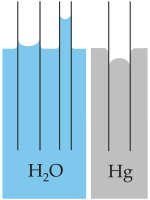
\includegraphics[height=0.15\textheight]{capillarity.png}
\caption[https://de.wikipedia.org/wiki/Kapillarität]{Kapillarität \\ H2O \dots Wasser \quad Hg \dots Quecksilber}
\end{figure}
~\\
Kapillarität ist das Verhalten, welches Flüssigkeiten bei engen Röhren, Spalten oder Hohlräumen in Feststoffen zeigen.
Dieses wird durch die Oberflächenspannung von Flüssigkeiten und der Grenzflächenspannung zum Festkörper hervorgerufen.

\newpage

\paragraph{Kapillaraszension}
Tritt bei Flüssigkeiten auf, die das Material des Kapillargefäßes benetzen, wie beispielsweise Wasser auf Glas oder auf Papierfasern.
Das Wasser steigt aufgrund der Adhäsionskraft\footnote{Kraft, die zwischen zwei Stoffen wirkt} in einem Glasröhrchen auf und bildet eine konkave Oberfläche.

\paragraph{Kapillardepression}
Tritt auf, wenn die Flüssigkeit das Material der Gefäßoberfläche nicht benetzt.
Quecksilber zum Beispiel hat in einem Röhrchen einen niedrigeren Pegel als in der Umgebung und eine konvexe Oberfläche.

\paragraph{Formel}
Die Steighöhe $h$ einer Flüssigkeitssäule ist gegeben durch
$$h = \frac{2\gamma \cos{\theta}}{\rho * g * r}$$
Ohne Neigung $\Theta = 0$ entspricht dies
$$h = \frac{2\gamma}{\rho * g * r}$$

\begin{center}
    \begin{tabular}{l l l}
        $\gamma$ &\dots Oberflächenspannung & $\frac{J}{m^2}$\\
        $\Theta$ &\dots Kontaktwinkel & $rad$\\
        $\rho$ &\dots Länge & $\frac{kg}{m^3}$\\
        $g$ &\dots Erdbeschleunigung & $9.81\frac{m}{s^2}$\\
        $r$ &\dots Radius & $m$
    \end{tabular}
\end{center}

\newpage
\subsubsection{Bsp.: Wasserhahn}
Auf einem Wasserhahn mit einem Durchmesser von $3mm$, hat sich ein Wassertropfen gebildet.
Berechne den Durchmesser des Tropfens.
\begin{center}
    \begin{tabular}{l l l}
        Dichte Wasser & $\rho_{H2O}$ & $1000 \frac{kg}{m^3}$\\
        Oberflächenspannung Wasser & $\gamma_{H2O}$ & $0.07 \frac{N}{m}$\\
        Umfang Zylinder & $U_{Zylinder}$ & $2*r*\pi$\\
        Volumen Kugel & $V_{Kugel}$ & $\frac{4*\pi*r^3}{3}$
    \end{tabular}
\end{center}
Die Kraft welche nach Unten wirkt bildet sich aus der Masse des Tropfens und der Erdbeschleunigung $G = m*g$ mit $g = 9.81$.
\vspace{0.8 em}\\
Die Nach oben wirkende Kraft ist die Oberflächespannung im Hahn $\gamma_{H2O} = F * U_{Zylinder}$.
\vspace{0.8 em}\\
Durch umformen kommt man damit auf folgende Gleichungen.
$$F_\uparrow = U_{Zylinder} * \gamma_{H2O}$$
$$G_\downarrow = V_{Kugel} * \rho_{H2O} * g$$
Damit der Wassertropfen am Hahn erhalten bleibt müssen sich die Kräfte die nach oben wirken und jene die nach unten wirken aufheben $F_\uparrow = G_\downarrow$.
$$U_{Zylinder} * \gamma_{H2O} = V_{Kugel} * \rho_{H2O} * g$$
$$2*r_{Zylinder}*\pi * \gamma_{H2O} = \frac{4*\pi*{r_{Kugel}}^3}{3} * \rho_{H2O} * g$$
$$2*1.5*\pi*0.07 = \frac{4}{3}*\pi*{r_{Kugel}}^3 * 1000 * 9.81$$
Nun kann man einfach auf $r_{Kugel}$ umformen und das Ergebnis in die Formel für den Umfang einsetzen.
$$r \approx 2.757mm$$
$$U_{Kugel} = 2*\pi*r \approx 18.847mm$$

\newpage
\section{Elektrische Leistung in Festkörpern}
\subsection{Bändermodell}
Im Bändermodell liegen mehrere Energiebereiche mit verschiedenen Zuständen energetisch dicht beieinander.
Diese Bereiche werden Energiebänder genannt.

\begin{figure}[!ht]
\centering
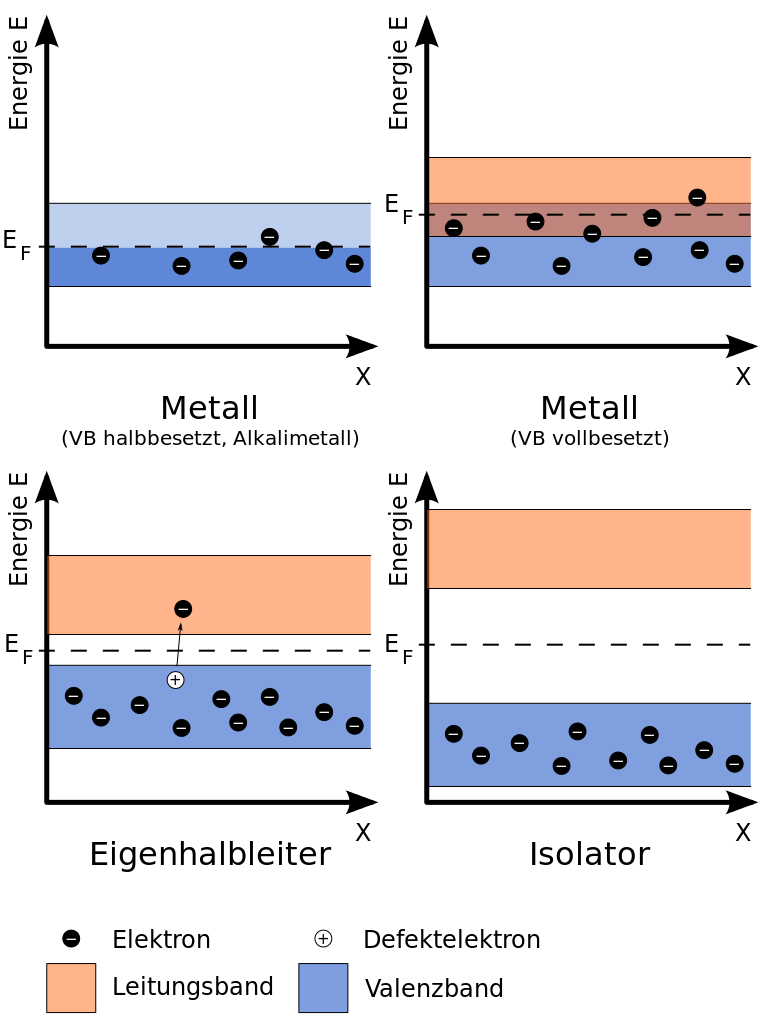
\includegraphics[width=0.4\textwidth]{baendermodell.png}
\caption[https://de.wikipedia.org/wiki/Bändermodell]{Bändermodell}
\end{figure}
~\\
Halbbesetzte Metalle werden auch \textbf{einwertig} und vollbesetzte Metalle \textbf{zweiwertig} genannt.

\subsubsection[Ferminiveau]{Ferminiveau $E_F$}
Das Farminiveau beschreibt den Bereich, bis zu welchem sich Elektronen frei bewegen können.
Der Abstand zwischen dem Niveau und den Bändern wird als Bandlücke bezeichnet und in $eV$\footnote{$eV \text{\dots Elektronenvolt}$ beschreibt die kinetische Energieänderung bei einem Volt.} angegeben.
\paragraph{Isolator}
Die Bandlücke ist größer als $2.5eV$, weshalb kaum Elektronen angeregt werden.
\paragraph{Halbleiter}
Die Bandlücke ist kleiner als $2.5eV$ und wird durch Energiezufuhr überbrückt.
\paragraph{Einwertige Metalle}
Das Leitungsband liegt auf dem Ferminiveau, wodurch Elektronen bereits bei geringer Energiezufuhr angeregt werden.
\paragraph{Zweiwertige Metalle}
Valenz- und Leitungsband überlappen am Ferminiveau und Elektronen werden immer werden.

\newpage
\section{Aufbau der Materie}
\subsection{Bohr'sches Atommodell}
Atome bestehen bei diesem Modell aus einem positiv geladenen Atomkern und negativ geladenen Elektronen, die den Atomkern auf geschlossenen Bahnen umkreisen.\cite{wikipedia-bohr}

\begin{figure}[!ht]
\centering
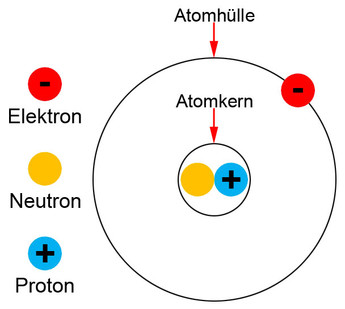
\includegraphics[width=0.25\textwidth]{einfaches-atommodell-a3.jpg}\\
\caption[https://www.sps-lehrgang.de/atommodelle/]{Bohr'sches Atommodell}
\end{figure}

\subsubsection[Bohr'sche Postulate]{Bohr'sche Postulate\protect\footnote{Eine wissenschaftliche Annahme oder Behauptung}}
\begin{enumerate}
    \item Elektronen umkreisen strahlungsfrei den Atomkern
    \item Beim Übergang von Elektronen zwischen zwei Elektronenbahnen wird Energie abgestrahlt oder aufgenommen
\end{enumerate}

\subsubsection{Festkörper}
Bei Festkörpern sind Atome in einem Kristallgitter angeordnet.
Stahl, als Beispiel, hat im Eisengitter ein C-Atom angeordnet.

\begin{figure}[!ht]
    \centering
    \begin{subfigure}[!ht]{0.2\textwidth}
        \centering
        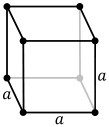
\includegraphics[width=0.6\textwidth]{cubic.png}
        \caption[https://de.wikipedia.org/wiki/Bravais-Gitter]{Primitiv}
    \end{subfigure}
    \begin{subfigure}[!ht]{0.2\textwidth}
        \centering
        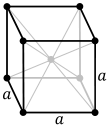
\includegraphics[width=0.6\textwidth]{cubic-centered.png}
        \caption[https://de.wikipedia.org/wiki/Bravais-Gitter]{Raumzentriert}
    \end{subfigure}
    \begin{subfigure}[!ht]{0.2\textwidth}
        \centering
        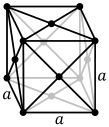
\includegraphics[width=0.6\textwidth]{cubic-face-centered.png}
        \caption[https://de.wikipedia.org/wiki/Bravais-Gitter]{Flächenzentriert}
    \end{subfigure}
    \caption[https://de.wikipedia.org/wiki/Bravais-Gitter]{Kubische Gitter}
\end{figure}

\begin{enumerate}[label= (\alph*)]
    \item \textbf{Kubisch primitives Gitter} Es ist kein weiteres C-Atom enthalten
    \item \textbf{Kubisch raumzentriertes Gitter} Das C-Atom befindet sich im Zentrum
    \item \textbf{Kubisch flächenzentriertes Gitter} Jede Fläche enthälft ein C-Atom in der Mitte
\end{enumerate}

\newpage
\section{Relativistische Mechanik}
Klassische Mechanik $v << c$\hfill$c$ \dots Lichtgeschwindigkeit\\
Relativistische Mechnanik $v < c$

\subsection{Galileo Transformation}
$[x, y, z]$ Ruhiges System $S$\\
$[x', y', z']$ Bewegtes System $S'$

\begin{figure}[!ht]
\centering
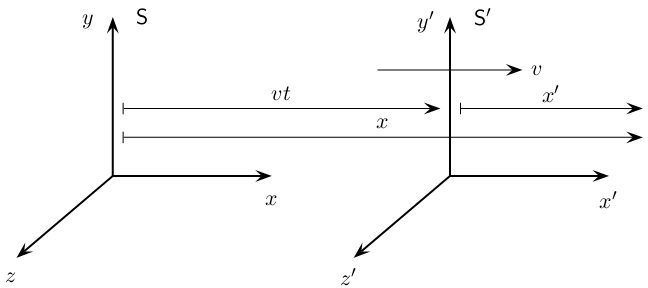
\includegraphics[width=0.8\textwidth]{galileo-transformation.png}\\
\caption[http://html.smartpub.dk/egaagymnasium/infogeist\--eg12\--fy/]{Galileo Transformation}
\end{figure}
\begin{center}
    $\Rightarrow$ Zeit und Beschleunigung bleiben gleich, Geschwindigkeit ändert sich
\end{center}

\begin{tabular}{l l l l}
    $t = t' \rightarrow$ Zeit bleibt gleich & $t$ &\dots Zeit & $s$\\
    $x = x' + v*t \rightarrow$ Geschwindigkeit ändert sich & $v$ &\dots Geschwindigkeit & $\frac{m}{s}$\\
\end{tabular}

\paragraph{Geschwindigkeit}
$$u_{x} = \frac{dx}{dt}$$
$$u_{x}' = \frac{d(x - v*t)}{dt} = u_x - v$$

\paragraph{Beschleunigung}
$$a = \frac{du}{dt} = \frac{du * x}{dt}$$

\begin{center}
    \begin{tabular}{l l l}
        $a$ &\dots Beschleunigung & $\frac{m}{s^2}$\\
        $du$ &\dots Geschwindigkeitsänderung & $\frac{m}{s}$\\
        $dx$ &\dots Positionsänderung & $m$\\
        $dt$ &\dots Zeitänderung & $s$
    \end{tabular}
\end{center}

\newpage
\section{Relativitätstheorie}
\subsection[Speziell]{Spezielle Relativitätstheorie \small{(Abhängig von Geschwindigkeit)}}
Für bewegte Objekte vergeht die Zeit langsamer\\
Bewegte Objekte verringern ihr Volumen und erhöhen Masse

\subsection[Allgemein]{Allgemeine Relativitätstheorie \small{(Abhängig von Gravitation)}}
Unter Einwirkung von Gravitation vergeht die Zeit langsamer\\
Unter Einwirkung von Gravitation verringern Körper ihr Volumen und erhöhen ihre Masse

\subsection{Lorentz Transformation}
Verbindet in der speziellen Relativitätstheorie die Zeit- und Ortskoordinaten, mit denen verschiedene Beobachter angeben, wann und wo Ereignisse stattfinden.

\paragraph{Ortskoordinaten}
$$x' = \frac{x - v * t}{\sqrt{1 - \frac{v^2}{t^2}}}$$
\paragraph{Zeitkoordinaten}
$$t' = \frac{t - v * \frac{x}{c^2}}{\sqrt{1 - \frac{v^2}{t^2}}}$$
\paragraph{Relativistische Geschwindigkeitsaddition}
$$v_x = \frac{v_x' + v}{1 + \frac{v_x' * v}{c^2}}$$

\begin{center}
    \begin{tabular}{l l l}
        $t$ &\dots Zeit & $s$\\
        $v$ &\dots Geschwindigkeit & $\frac{m}{s}$\\
        $c$ &\dots Lichtgeschwindigkeit & $3*10^8 \frac{m}{s}$
    \end{tabular}
\end{center}

\newpage
\subsection[Zeitdelitation]{Zeitdelitation\footnote{Delitation (lat.\ verlängern, ausdehnen) der Zeit}}
Alle inneren Prozesse eines physikalischen Systems scheinen langsamer abzulaufen, wenn sich dieses System relativ zum Beobachter bewegt.

\paragraph{Formel}
$$t_2' = t_1' + \Delta t' = \frac{t_2 - t_1}{\sqrt{1 - \frac{v^2}{c^2}}}$$
$$\Delta t' = \frac{\Delta t}{\sqrt{1 - \frac{v^2}{c^2}}}$$
\vspace{0.8 em}

\subsubsection{Bsp.: Zwillingsparadoxon}
Während ein Zwilling auf der Erde bleibt, bewegt sich der andere mit 60\% der Lichtgeschwindigkeit $v = 0.6 * c$.
Welche Zeit vergeht für den Zwilling im All nach 4 Jahren auf der Erde?
$$\Delta t = \Delta t' * \sqrt{1 - \frac{v^2}{c^2}}$$
$$\Delta t = 4 * \sqrt{1 - \frac{{(0.6 * c)}^2}{c^2}}$$
$$\Delta t = 3.2 \text{Jahre}$$
\vspace{0.8 em}\\
Für den Zwilling auf der Erde sind also 4 Jahre vergangen, der Zwilling im All erlebte jedoch nur 3.2 Jahre.

\subsubsection{Bsp.: Raumstation}
Mit welcher Geschwindigkeit müsste sich ein Beobachter relativ zur Erdstation bewegen, damit damit für diesen 10 Jahre auf der Erde in einem Jahr vergehen?
$$\Delta t' = \frac{\Delta t}{\sqrt{1 - \frac{v^2}{c^2}}}$$
$$10 = \frac{1}{\sqrt{1 - \frac{v^2}{c^2}}}$$
$$v = \sqrt{1 - {(\frac{1}{10})}^2 * c^2}$$
\vspace{0.8 em}
$$v = 0.\overline{9} * c \approx 99\% \text{ der Lichtgeschwindigkeit}$$

\newpage
\subsection[Längenkontraktion]{Längenkontraktion\footnote{Kontraktion (lat.\ verkleinern, zusammenziehen) des Raums}}
Ein bewegter Beobachter misst eine kürzere Distanz zwischen zwei Punkten im Raum als ein ruhender.

\paragraph{Formel}
$$l' = (x_2 - x_1) * \sqrt{1 - \frac{v^2}{c^2}}$$
$$\Delta l = \frac{l'}{\sqrt{1 - \frac{v^2}{c^2}}}$$
\vspace{0.8 em}
$$l = (x_2' - x_1') * \sqrt{1 - \frac{v^2}{c^2}}$$
$$\Delta l' = \frac{l}{\sqrt{1 - \frac{v^2}{c^2}}}$$

\subsubsection{Bsp.: Würfel}
Im System $S'$ liegt ein Würfel mit der Kantenlänge $a'$
\begin{enumerate}
    \item Welches Volumen misst ein Beobachter im System $S$, wenn sich $S'$ mit der Geschwindigkeit $v$ bewegt?
    $$V' = a^3 * \sqrt{1 - \frac{v^2}{c^2}}$$
    \item Welche Dichte misst der Beobachter?
    $$\rho' = \frac{m'}{V'} = m * a^3 * \sqrt{1 - \frac{v^2}{c^2}}$$
\end{enumerate}

\newpage
\subsubsection{Bsp.: Einsteinzug}
Der Einsteinzug ist $330$ Meter lang und fährt mit einer Geschwindigkeit von $v = 0.8c$.
Ein Fahrgast am Zugende gibt einen Schuss mit $v = 0.6c$ ab.
\begin{enumerate}
    \item Welche Geschwindigkeit misst ein Beobachter?
    \item Welche Zuglänge misst er?
\end{enumerate}
$$v_x = \frac{v_x' + v}{1 + \frac{v_x' * v}{c^2}}$$
$$v_x = \frac{0.6c + 0.8c}{1 + \frac{0.8c * 0.6c}{c^2}}$$
$$v_x = \frac{1.4c}{1.48} \approx 0.95c$$
\\
Der Beobachter misst eine Geschwindigkeit von 95 Prozent der Lichtgeschwindigkeit
$$\Delta l' = \frac{l}{\sqrt{1 - \frac{v^2}{c^2}}}$$
$$\Delta l' = \frac{330}{\sqrt{1 - \frac{0.95c^2}{c^2}}} \approx 1475.8m$$
\\
Der Beobachter misst eine Länge von 1475.8 Meter

\newpage
\section{Quantenphysik}
Nach Max Planck, ist jede Strahlung aus Quanten zusammengesetzt. Quanten sind Objekte, welche durch einen Zustandswechsel (meist Energie) erzeugt werden.

\subsection{Plancksches Wirkungsquantum}
Das Planksche Wirkungsquantum $h$, beschreibt das Verhältnis von Energie $E$ und Frequenz $f$ eines Photons\footnote{In diesem Kontext auch als Lichtquant bekannt}.
$$E = h * f$$
$$f = \frac{c}{\lambda}$$
\begin{center}
    \begin{tabular}{l l l}
        $h$ &\dots Wirkungsquantum & $6.63 * 10^{-34} Js$\\
        $f$ &\dots Frequenz & ${s}$\\
        $f$ &\dots Wellenlänge & ${m}$
    \end{tabular}
\end{center}

\subsubsection{Bsp.: Masse eines Photons}
Einsteins Äquivalenzenprinzip und das Plancksche Wirkungsquantum können gleichgesetzt werden, womit sich die Masse eines Photons, bei einer bestimmten Wellenlänge (hier $500nm$) errechnen lässt.
$$E = m * c^2$$
\begin{center}
    \begin{tabular}{l l l}
        $E$ &\dots Energie & $J$\\
        $m$ &\dots Masse & $kg$\\
        $c$ &\dots Lichtgeschwindigkeit & $3*10^8 {m}{s^2}$
    \end{tabular}
\end{center}
\vspace{0.8 em}
$$h * f = m * c^2$$
$$m = \frac{6.63 * 10^{-34} * 500 * 10^{-9}}{c^2}$$
$$m \approx 44.2 * 10^{-34}g $$

\newpage
\subsection{Bsp.: Fotozelle}
Eine Fotozelle spricht an, wenn sie mit Licht der Leistung $P = 10^{-18}$ Watt bestrahlt wird.
Wie viele Lichtquanten $N$ (Photonen) der Wellenlänge $\lambda = 6.44 * 10^{-7}$ Meter fallen pro Sekunde auf die Fotozelle?
$$E = P*t$$
Die Energie gilt der Anzahl der Photonen $N$, diese wird einfach als Faktor des Wirkungsquantum hinzugefügt.
$$E = N * h*f$$
$$f = \frac{c}{\lambda}$$
$$P*t = N * \frac{h * c}{\lambda}$$
$$N = \frac{P*t*\lambda}{h*c}$$
$$N = \frac{10^{-18}*1*6.44*10^{-7}}{6.63*10^{-34}*3*10^8}$$
\vspace{0.8 em}
$$N \approx 3.238 \text{ Lichtquanten}$$

\subsubsection{Bsp.: Glühbirne}
5 Prozent der elektrischen Leistung einer 60 Watt Glühbirne, wird in Licht der Wellenlänge $\lambda = 5.6 * 10^{-7}$ Meter umgewandelt.
Wie viele Lichtquanten dieser Wellenlänge werden pro Sekunde ausgesandt?
$$N = \frac{P*t*\lambda}{h*c}$$
$$N = \frac{60*1*5.6*10^{-7}}{6.63*10^{-34}*3*10^8}$$
\vspace{0.8 em}
$$N \approx 0.43*10^{18} \text{ Lichtquanten}$$

\newpage
\subsection{Unschärferelation}
Jede Steigerung der Genauigkeit in der Ortsbestimmung reduziert die Genauigkeit in der Geschwindigkeitsbestimmung.
\vspace{0.8 em}\\
Diese Ungenauigkeit ist prinzipieller Natur und kann durch verbesserte Technologien nicht reduziert werden.\\
Die Unschärferelation gilt auch für makroskopische Körper.
\paragraph{Heisenberg}
$$\Delta x * \Delta p \ge \frac{h}{2\pi}$$
\vspace{0.25 em}
$$p = m * v$$

\begin{center}
    \begin{tabular}{l l l}
        $h$ &\dots Plancksches Wirkungsquantum & $6.63 * 10^{-34} Js$\\
        $p$ &\dots Impuls & ${kg*m}{s}$\\
        $m$ &\dots Masse & ${kg}$\\
        $v$ &\dots Geschwindigkeit & ${m}{s}$\\
        $\Delta x$ &\dots Unschärfe des Ortes & ${m}$\\
        $\Delta p$ &\dots Unschärfe des Impulses & ${kg*m}{s}$
    \end{tabular}
\end{center}

\subsubsection{Bsp.: Auto}
Ein Auto mit der Masse $m = 1200 kg$ bewegt sich mit $v = 170 \frac{km}{h}$.
Welche Ungenauigkeit tritt bei der Bestimmung des Ortes mindestens auf?
$$\Delta x * \Delta p \ge \frac{h}{2\pi}$$
Der Impuls kann in diesem Fall genau über $m * v$ bestimmt werden, da es sich um die minimale Ungenauigkeit handelt wird das $\ge$ zu einem $=$.
$$\Delta x = \frac{h}{2\pi * m * v}$$
$$\Delta x = \frac{6.63 * 10^{-34}}{2\pi * 1200 * \frac{170}{3.6}}$$
$$\Delta x \approx 1.76 * 10^{-39} m$$

\newpage
\section{Weiteres}
\subsection{Beleuchtung}
\paragraph{Glühlampe}~\\
Temperatur $1500^\circ - 3000^\circ$ Celsius\\
Ca. 5\% der Energie wird in Licht, der Rest in Wärme umgewandelt
\paragraph{Leuchtstoffröhre (Energiesparlampe)}

\begin{figure}[!ht]
\centering
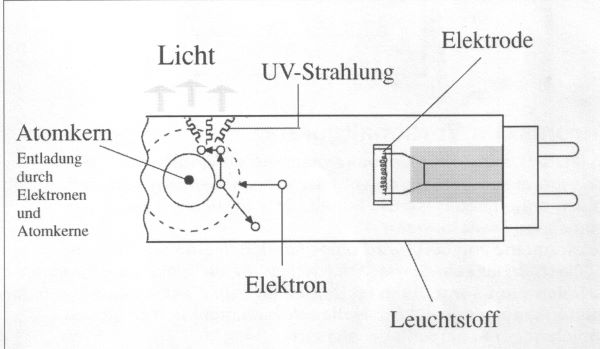
\includegraphics[width=0.4\textwidth]{leuchtstoff.jpg}\\
\caption[http://basics-de.de/Lexikon/GluehlampenBatterien]{Aufbau einer Leuchtstoffröhre}
\end{figure}
~\\
Netzfrequenz $50$ Hertz\\
Es tritt kein Flackern auf, da der Leuchtstoff selbst leuchtet

\paragraph{Schwarzlicht Lampen}~\\
Strahlen im UV Bereich $\to$ weißer Stoff beginnt zu leuchten

\paragraph{Leuchtdiode LED}~\\
Die LED (Light Emitting Diod) wandelt besonders viel Energie in Licht um

\newpage
\begin{thebibliography}{9}
    \bibitem{wikipedia-baendermodell} https://de.wikipedia.org/wiki/Bändermodell
    \bibitem{wikipedia-bohr} https://de.wikipedia.org/wiki/Bohrsches\_Atommodell
    \bibitem{wikipedia-atomrumpf} https://de.wikipedia.org/wiki/Atomrumpf
    \bibitem{wikipedia-capillarity} https://de.wikipedia.org/wiki/Kapillarität
    \bibitem{zwillingsparadoxon} http://www.leifiphysik.de/relativitaetstheorie/spezielle-relativitaetstheorie
\end{thebibliography}

\listoffigures

\end{document}
